% generated by experiments/build_paper_assets.py -- do not edit by hand
\begin{figure}[t]
\centering
\resizebox{\linewidth}{!}{%
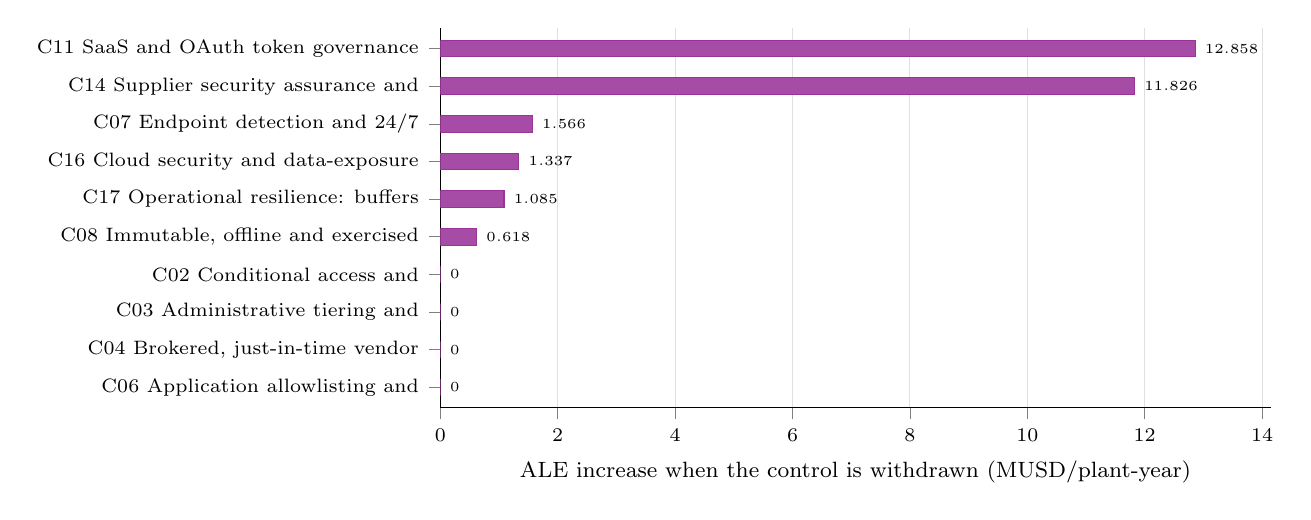
\begin{tikzpicture}
\begin{axis}[
    xbar, width=\linewidth, height=6.4cm,
    xlabel={ALE increase when the control is withdrawn (MUSD/plant-year)},
    xmin=0, enlarge y limits=0.06,
    ytick={0,1,2,3,4,5,6,7,8,9}, yticklabels={{C11 SaaS and OAuth token governance},{C14 Supplier security assurance and},{C07 Endpoint detection and 24/7},{C16 Cloud security and data-exposure},{C17 Operational resilience: buffers},{C08 Immutable, offline and exercised},{C02 Conditional access and},{C03 Administrative tiering and},{C04 Brokered, just-in-time vendor},{C06 Application allowlisting and}},
    y dir=reverse, ticklabel style={font=\scriptsize},
    label style={font=\footnotesize},
    nodes near coords, nodes near coords style={font=\tiny},
    every node near coord/.append style={/pgf/number format/fixed,
        /pgf/number format/precision=3},
    xmajorgrids, grid style={gray!25}, axis lines*=left,
    bar width=6pt, tick align=outside,
]
\addplot[fill=Purple!70, draw=Purple!80] coordinates {
        (12.858000,0)
        (11.826000,1)
        (1.566000,2)
        (1.337000,3)
        (1.085000,4)
        (0.618000,5)
        (0.000000,6)
        (0.000000,7)
        (0.000000,8)
        (0.000000,9)
};
\end{axis}
\end{tikzpicture}}
\caption{Necessity of each control inside the full programme $S_5$: the annualised loss that returns when that control alone is withdrawn.}
\label{fig:necessity}
\end{figure}
